% Appendix A

\chapter{Lorentz angle measurement in Pixel detector} % Main appendix title

\label{AppendixA} % For referencing this appendix elsewhere, use \ref{AppendixA}

\lhead{Appendix A. \emph{Lorentz angle measurement in Pixel detector}} 

\section{Grazing angle method}
Lorentz angle is measured by using grazing angle method described in detail in \cite{Henrich}. From the individual signals in the detector, using reconstruction algorithms, tracks of muon candidates are obtained. From these reconstructed track it is possible to extract the entry point ($x_{reco}$,$y_{reco}$) to each layer of the detector. 
Distance between reconstructed entry point and the actual hit in the detector is then defined as ($\Delta x$,$\Delta y$):
\begin{equation}
\Delta x = x_{center}-x_{reco}
\end{equation} 
\begin{equation}
\Delta y = y_{center}-y_{reco}
\end{equation} 

where ($x_{center}$,$y_{center}$) is the position of each individual pixel center in the observed cluster. Drift of the electrons can be determined using three impact angles defined in the following way:

\begin{equation}
\text{tan} \alpha = \frac{p_z}{p_x}
\end{equation}
\begin{equation}
\text{tan} \beta = \frac{p_z}{p_y}
\end{equation}
\begin{equation}
\text{tan} \gamma = \frac{p_x}{p_y}
\end{equation}

where $p_x$,$p_y$ and $p_z$ are momentum components in local coordinate system which are calculated from reconstructed track parameters (Fig. \ref{fig:kut}). \\
\begin{figure}[ht!]
\centering
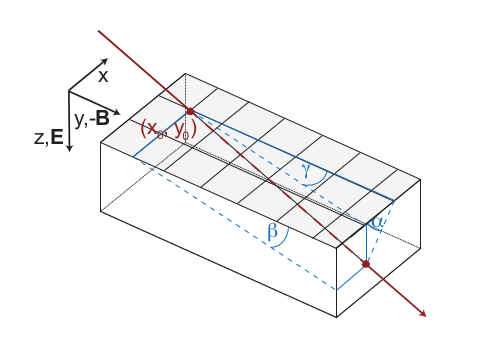
\includegraphics[width=0.5\textwidth]{Figures/kut.png}
\caption{Angle definitions for grazing angle method.}
\label{fig:kut}
\end{figure}
Drift of the electrons depends on the depth at which electrons are created. Depth of the electron production $z$ and drift due to magnetic field $d$ are defined:

\begin{equation}
z = \Delta y \text{ tan}\beta
\end{equation}
\begin{equation}
d=\Delta x-\Delta y \text{ tan}\gamma
\end{equation}

This procedure is repeated for each pixel over many tracks in order to obtain charge drift distance vs depth. The Lorentz angle is the slope of this distribution.  Without a magnetic field, the
direction of the clusters largest extension is parallel to the track projection on the (x, y) plane. The average drift distance of an electron created at a certain depth is obtained from Fig. \ref{fig:2D}. A linear fit is
performed over the total depth of the detector excluding the first and last 50 $\mu$ where the charge drift is systematically displaced by the finite size of the pixel cell (Fig:\ref{fig:profile}). 

\begin{figure}[ht!]
\centering
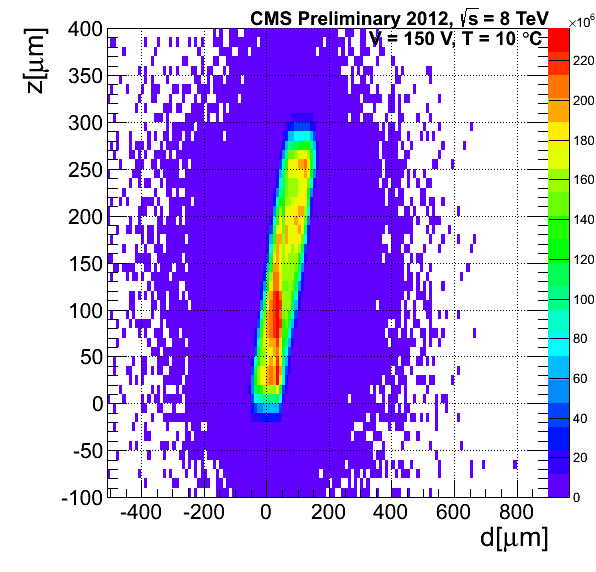
\includegraphics[width=0.5\textwidth]{Figures/LA2012_2D.png}
\caption{Depth at which electrons in silicon bulk were produced as a function of Lorentz drift.}
\label{fig:2D}
\end{figure}

\begin{figure}[ht!]
\centering
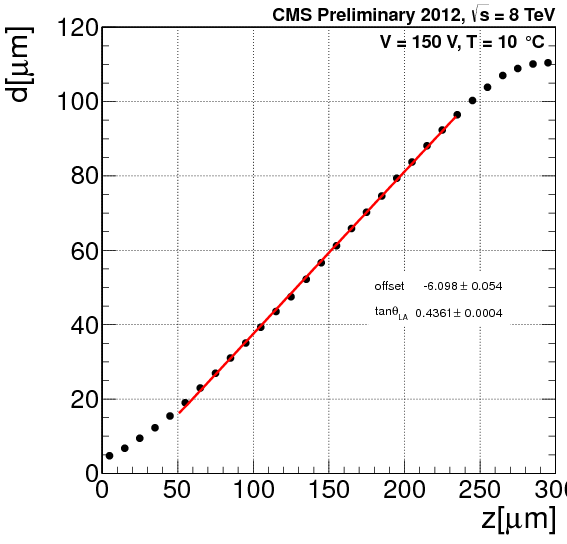
\includegraphics[width=0.5\textwidth]{Figures/LA2012_Profile.png}
\caption{The average drift of electrons as a function of the production depth. Slope of the linear fit result is the $tan \theta_L$.}
\label{fig:profile}
\end{figure}

In order to obtain a good measurement, it is important to use clean tracks. Therefore, it required to have a well reconstructed muon tracks with $p_T>3$GeV and $\chi^2/ndof<2$ which are required to have shallow impact angle with respect to local $y$ direction with cluster size of at least 4 pixels in this direction. Summary of the selection criteria can be found in table \ref{tab:sel}.

\begin{table}[ht!]
  \caption{Selection criteria for Lorentz angle measurement}
  \centering
  \begin{tabular}{l|c}
\hline
\hline
        Cluster size in y & $>3$  \\
	Track $p_t$ & $>3$GeV$/$c \\
	$\chi^2$/ndof & $<2$ \\
	Hit residuals & $<50\mu m$ \\
	Cluster charge & $<120000$e \\
\hline
\hline
  \end{tabular}
  \label{tab:sel}
\end{table}

Figure \ref{fig:La2012} shows how Lorentz angle changes with integrated luminosity. Results are shown for 23fb$^{-1}$ of delivered luminosity in 2012. Increase in Lorentz angle measured with grazing angle method has been observed in all layers, with largest effect (~6\%) visible in layer 1 over this period of data taking.  
\begin{figure}[ht!]
\centering
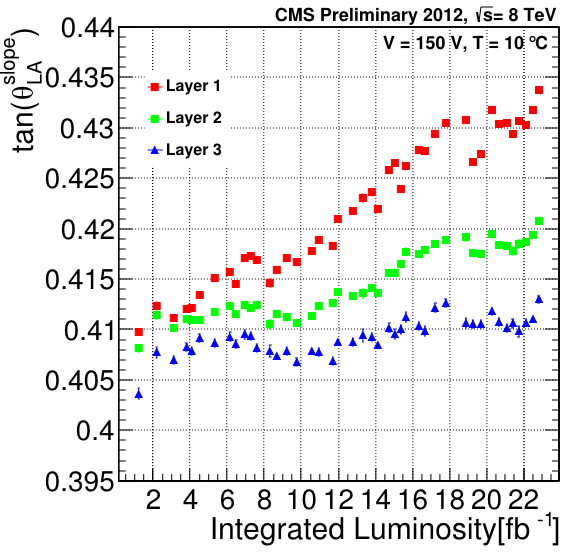
\includegraphics[width=0.5\textwidth]{Figures/LA2012.png}
\caption{Lorentz angle as a function of integrated luminosity for 2012.}
\label{fig:La2012}
\end{figure}

\section{Minimum cluster size method (V-method)}
The pixel cluster size in the drift direction depends on the incident
angle and is minimal when incident angle is equal to the Lorentz angle. Thus, measuring the average cluster size in drift direction as a function of incident angle and obtaining a minimum of that
distribution is an alternative and direct method of measuring the Lorentz angle. The method is usually referred to as V-method due
to a shape of distribution which in the simple case can be approximated with formula

\begin{equation}
p_1*abs(tan(\theta) - p_0) + p_2
\end{equation}
where $p_0$, $p_1$ and $p_2$ are parameters obtained from the fit and $p_0$ = $tan(\theta_{LA})$.

The method was successfully applied to cosmic muon tracks during CMS commissioning period in 2008 and again in 2015. The fit result is shown in figure \ref{fig:LA_VMethod}.

\begin{figure}[hbtp!]
	\centering
	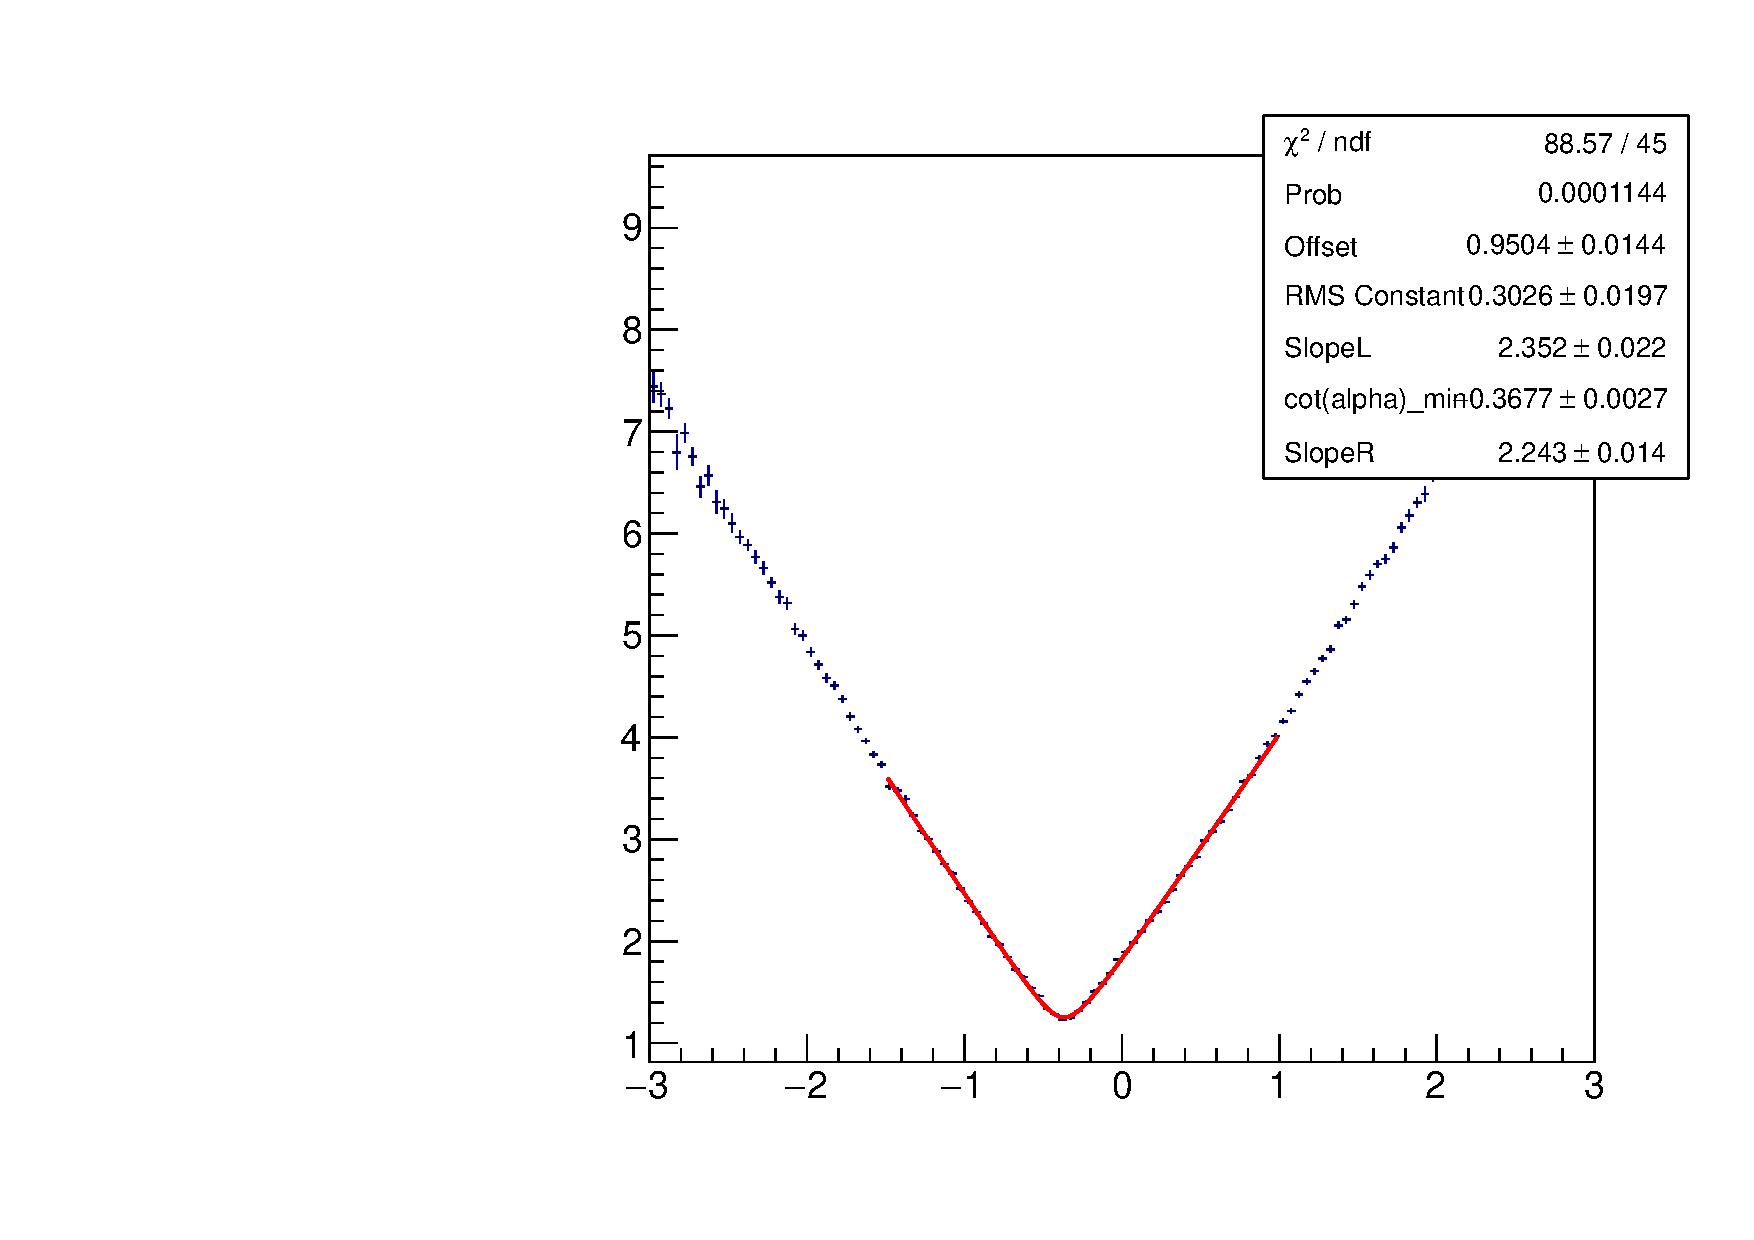
\includegraphics[width=0.5\textwidth]{Figures/LA_VMethod_2015.pdf}
\end{figure}

Application to collision data is more challenging. Coordinates of a track passing through the detector, its incoming angle, and its $p_T$ are
correlated and therefore incoming angles from collision tracks have limited range. With
standard running conditions the value of Lorentz angle is at the edge of that range where tracks with very low $p_T$ (<0.5 GeV) dominate. Because
of that average cluster size as a function of incoming angle cannot be described by a simple model like above mentioned for cosmic data.
While  results for collision data obtained with V-method are in general agreement with the default calculation,  the uncertainty of
the method at present is too big to be used as a viable alternative.

